\documentclass[11pt,addpoints]{exam}
\printanswers

\usepackage{amsmath}
\usepackage{amssymb}
\usepackage{bm}

\usepackage{graphicx}
\usepackage[usenames,dvipsnames]{color}

\usepackage[utf8]{inputenc}
\usepackage[T1]{fontenc}
\usepackage{lmodern} % load a font with all the characters


% Bold the 'Figure #' in the caption and separate it with a period
% Captions will be left justified
\usepackage[labelfont=bf,labelsep=period,justification=raggedright]{caption}
%\usepackage{here}

\title{Examen Cours ES2: Introduction à la bioinformatique et la génomique}
\author{Chloé-Agathe Azencott, Thomas Walter}
\begin{document}
\maketitle 

\begin{questions}

\section{Questions sur le cours}

\question[2] Notions en Biologie. 
\begin{parts}
\part Citer trois fonctions de protéines. 
\part Expliquer pourquoi un codon est constitué de trois nucléotides. 
\part Expliquer le principe de l'interférence par ARN.
\part Classer les mutations selon leur effet. 
\end{parts}

\question[1] La microscopie.
\begin{parts}
\part Qu'est-ce qu'on entend par la résolution d'un microscope~? 
\part Décrire deux façons d'augmenter la résolution d'un microscope. 
\end{parts}

\question[3] Vous êtes consulté comme expert d'analyse d'images par
des biologistes qui veulent analyser une série d'expériences. Ils
utilisent un marqueur qui est informatif pour la compaction de la
chromatine, et ils cherchent à trouver des molécules spécifiques pour
rompre cette organisation. Dans les figure \ref{fig:tsa}.a et
\ref{fig:tsa}.b, nous pouvons observer des images représentatives pour
des cellules normales (sans traitement) et dans les figures
\ref{fig:tsa}.c et \ref{fig:tsa}.d nous pouvons observer l'effet d'une
molécule. Nous ajoutons que la taille et l'intensité moyenne des
cellules n'ont pas de raison d'être différentes entre les deux
conditions. 

Proposer un descripteur spécifique qui nous permettrait de quantifier
cet effet et expliquer votre choix. 

\begin{figure}[!ht]
\centering
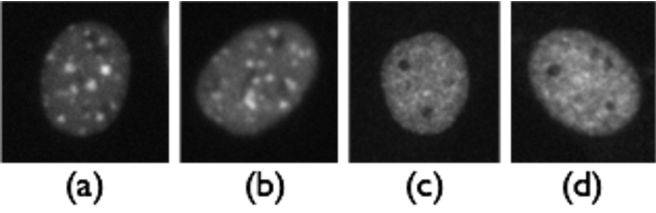
\includegraphics[scale=0.8]{TSA_phenotype.pdf}
\caption{Phenotypic readout on heterochromatin formation: (a)-(b)
  Negative Control, (c)-(d) Signal as observed 
  by an active drug.}
\label{fig:tsa}
\end{figure}

\question[4] Les descripteurs Haralick.
Les descripteurs de Haralick sont définis à partir de la matrice de
co-occurence normalisée $P_{\Delta_x}$. Nous rappelons que chaque élément
$P_{\Delta_x}(i,j)$ de cette matrice est la probabilité jointe
d'observer les valeurs de gris $i$ et $j$ pour des paires de pixels
$(x,x+\Delta_x)$ et $(x,x-\Delta_x)$, avec $Delta_x \in
\mathbb{Z}^2$. Plus formellement :  
\begin{eqnarray*}
C_{\Delta_x}(i,j) &=& |\{(x,y) \,\,| \,\, y=x \pm \Delta_x, \,\, f(x)=i,
\,\, f(y)=j \}| \\
P_{\Delta_x}(i,j) &=& \frac{C_{\Delta_x}(i,j)}{\sum_i\sum_j C_{\Delta_x}(i,j)}
\end{eqnarray*} 


Le descripteur de ``contraste'' est défini de manière suivante: 
\begin{equation}\label{equ:haralick_contrast}
\vartheta_{\Delta_x} = \sum_i\sum_j(i-j)^2P_{\Delta_x}(i,j)
\end{equation}

\begin{parts}
\part Expliquer ce que le descripteur $\vartheta_{\Delta_x}$ mesure. 
\part Ordonner les images dans la figure \ref{fig:haralick} pour (i)
$\Delta_x=(1,0)$ et (ii) la matrice moyennée pour $\Delta_x\in
\{(1,0), (0,1)\}$ (c'est-à-dire en direction horizontale et
verticale).  

Par exemple, si le descripteur était ``le nombre de pixels noirs'', on
obtiendrait la solution 1. a - 2. (b,c,d,f) - 3. e. 
\end{parts}

\begin{figure}[!ht]
\centering
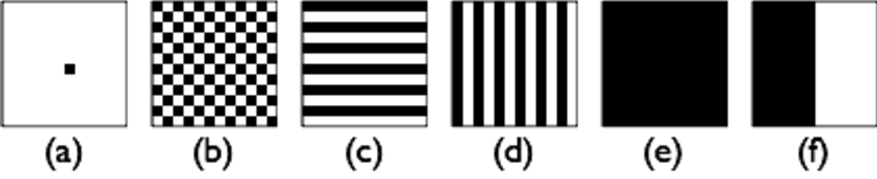
\includegraphics[scale=0.8]{Haralick_question.pdf}
\caption{Images à ordonner selon le descripteur
  \ref{equ:haralick_contrast} }. 
\label{fig:haralick}
\end{figure}


\question[4] Les chaines de Markov cachées. 
Beaucoup d'algorithmes autour des chaines de Markov cachées sont basés
sur le calcul récursif de certaines probabilités, dont : 
\begin{equation}\label{equ:alpha}
\alpha_t(i) = P(O_1\ldots O_t, q_t=S_i) 
\end{equation}
Ici, $O_t$ est l'observation au temps $t$, $q_t$ est l'état caché au
temps $t$ avec $q_t \in \{S_i\}_{i=1 \ldots N}$ (voire aussi figure
\ref{fig:hmm}).

\begin{parts}
\part Montrer que $\alpha_1(i)=\pi_i b_i(O_t)$. 
\part Montrer que $\alpha_{t+1}(j) = \left[
  \sum_{i=1}^{N}\alpha_t(i)a_{ij} \right]b_j(O_{t+1})$. 
\part Montrer que $P(O_1, \ldots O_{T}) = \sum_{i=1}^N\alpha_T(i)$. 

(Notation: $\pi_i = P(q_1=S_i)$ est la probabilité initiale pour état $S_i$,
$a_{ij} = P(q_{t+1}=S_j | q_t=S_i) $ la probabilité de transition,
$b_i(O_t) = P(O_t | q_t=S_i)$ la probabilité d'émission et $T$ la
longueur de la séquence.) 
\end{parts}

\begin{figure}[!ht]
\centering
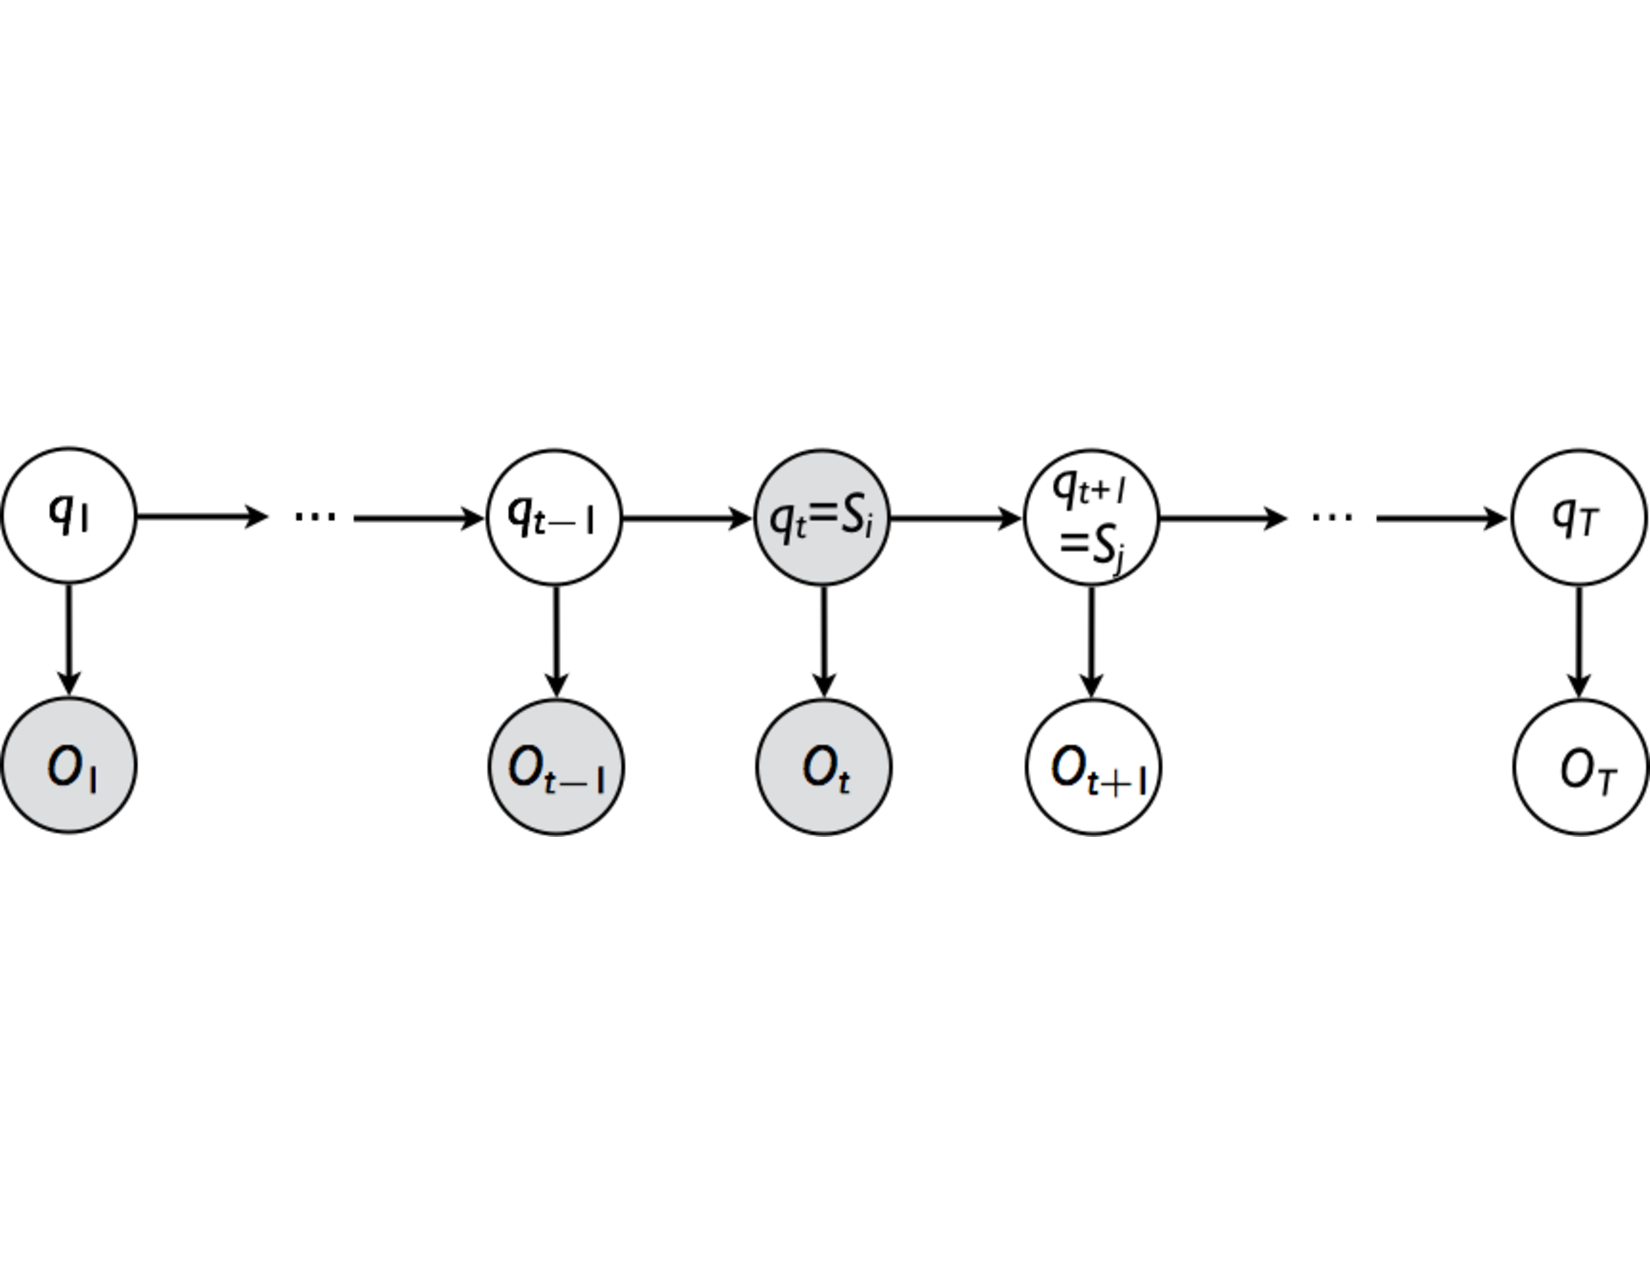
\includegraphics[width=12cm]{HMM.pdf}
\caption{Chaine de Markov cachée.}
\label{fig:hmm}
\end{figure}

%L'estimation des
%paramètres d'une chaine de Markov cachée à partir de séquences
%observées, est basée sur le calcul itératif de certaines probabilités,
%dont : 
%\begin{equation}\label{equ:beta}
%\beta_t(i) = P(O_{t+1}O_{t+2}\ldots O_T |q_t=S_i)
%\end{equation}
%Ici, $O_t$ est l'observation au temps $t$, $q_t$ est l'état caché au
%temps $t$ et $\{S_i\}_{i=1 \ldots K}$ est l'ensemble des états cachés. 

\section{Questions sur le papier ``Integrative clustering of multiple genomic data types using a joint latent variable model with application to breast and lung cancer subtype analysis.''}

\question[4] Il existe de nombreux algorithmes qui permettent de faire un clustering d'échantillons sur la base de mesures faites sur ces échantillons (par exemple, le niveau d'expression d'un grand nombre de gènes, ou leur nombre de copies).
\begin{parts}
\part Dans quel but cherche-t-on ici à faire du clustering d'échantillons de tumeurs ?
\begin{solution}
  Découvrir des sous-types de cancer.
\end{solution}
\part Quelle est la limitation de ces techniques que l'article se propose de corriger ?
\begin{solution}
  Impossibilité de faire ce clustering sur des sources de données multiples et hétérogènes.
\end{solution}
\part Quelles sont les deux difficultés rencontrées pour mettre en place cette nouvelle méthodologie ?
\begin{solution}
  \begin{itemize}
  \item Modéliser à la fois la covariance entre sources de données et la structure de variance-covariance au sein de chacune des sources.
  \item Réduire la dimension des données simultanément sur différents jeux de données corrélés.
  \end{itemize}
\end{solution}
\part Comment les différentes classes (clusters) d'échantillons sont-ils modélisés dans cette approche ?
\begin{solution}
  Comme des variables latentes / non-observées.
\end{solution}
\end{parts}

\question[2] Donner la dimension et l'interprétation des termes $\bm{W}$, $\bm{\Psi}$, $\bm{X}$ et $\bm{Z^*}$ dans l'Équation 9.
\begin{solution}
  \begin{itemize}
  \item $\bm{W}: (p_1 + p_2 + \dots + p_m) \times (K-1)$: matrice de projection qui associe l'espace des données à celui des $(K-1)$ directions principales sur lesquelles elles sont projetées.
  \item $\bm{\Psi}: (p_1 + p_2 + \dots + p_m) \times (p_1 + p_2 + \dots + p_m)$: matrice bloc-diagonale composée des matrices de covariance $\Psi_1, \dots, \Psi_m$ interne à chaque type de données.
  \item $\bm{X}: (p_1 + p_2 + \dots + p_m) \times n$: données.
  \item $\bm{Z^*}: (K-1) \times n$: version continue de la matrice $\bm{Z}$ qui assigne chaque échantillon à un cluster.
  \end{itemize}
\end{solution}

\question[3] Figure 2.   
\begin{parts}
\part Comment les auteurs utilisent-ils la Figure 2.B pour déterminer le nombre de clusters optimal ?
\part Quelle est la différence entre la Figure 2.A et la Figure 2.D~?
\part Que représentent les 3 lignes sur la Figure 2.E ? 
\end{parts}

\question[4] Figure 3
\begin{parts}
\part TODO
\end{parts}

\end{questions}

%\begin{enumerate}
%\item 
%\end{enumerate}
\end{document}
